\documentclass{article}
\usepackage{lmodern}
\usepackage{graphicx}
\usepackage{csquotes}
\usepackage[english]{babel}
\usepackage[colorlinks=true, allcolors=blue]{hyperref}

    \title{\textbf{Project Documentation}}
    \author{Andrei Suba, Silaghi-Fartan Stefan\\
	West University of Timișoara,\\
	Timișoara, Romania
    }
    \date{}
    
    \addtolength{\topmargin}{-3cm}
    \addtolength{\textheight}{3cm}

\usepackage{listings}
\usepackage{color}

\definecolor{dkgreen}{rgb}{0,0.6,0}
\definecolor{gray}{rgb}{0.5,0.5,0.5}
\definecolor{mauve}{rgb}{0.58,0,0.82}

\lstset{frame=tb,
  language=Python,
  aboveskip=3mm,
  belowskip=3mm,
  showstringspaces=false,
  columns=flexible,
  basicstyle={\small\ttfamily},
  numbers=none,
  numberstyle=\tiny\color{gray},
  keywordstyle=\color{blue},
  commentstyle=\color{dkgreen},
  stringstyle=\color{mauve},
  breaklines=true,
  breakatwhitespace=true,
  tabsize=3
}

\begin{document}

\maketitle
\thispagestyle{empty}

\begin{abstract}

\noindent In this paper, we present a small application written in Python that allows a user to interactively create points in two-dimensional space using their mouse. The application then computes the convex layers of the resulting point set and displays the resulting figure. The goal of this project was to develop a simple and intuitive tool for visualizing and understanding the concept of convex layers in a geometric context. The application is implemented using a combination of Python's built-in graphical user interface (GUI) library, Tkinter, and the Jarvis's Algorithm (or Gift Wrapping Algorithm) for computing the convex hull of points. We discuss the design and implementation of the application, as well as its potential applications in educational settings and beyond.

\end{abstract}

\clearpage

\tableofcontents

\clearpage

\section{Introduction}

Computational geometry is a crucial field in computer science that deals with the efficient representation and manipulation of geometric objects. One important concept in this field is the convex layer, which refers to the smallest convex polygon that encloses a given set of points in two-dimensional space. In this paper, we present a small application that allows users to interactively create points using their mouse and visualize the resulting convex layers in real-time. The application was developed using Python and makes use of the Tkinter library for the graphical user interface and the Jarvis's Algorithm for computing convex hulls. Our goal in creating this application was to provide a simple and intuitive tool for visualizing and understanding convex layers in a geometric context. In the following sections, we will describe the design and implementation of the application in detail and discuss its potential applications and future directions.

\section{Motivation}
A
s part of our university course on computational geometry, we were required to develop a project that demonstrated our understanding of the subject. We decided to focus on convex layers, as we felt that this was an important concept in the field. 
\newline
\newline
Our goal was to develop a simple and intuitive tool that would make the concept of convex layers more accessible and engaging for students and other learners. We believe that our small application has the potential to be a useful resource in educational settings where visualization makes for a better understanding. We hope that our project will provide a valuable learning experience for both ourselves and our users.

\section{Design and Implementation}

\subsection{Introduction}

In this chapter, we will discuss the technical details of the program that constructs the convex layers of a set of points. The user interface design, algorithm implementation and data structures will be explained. The goal of this chapter is to provide a clear understanding of the program's design and implementation and how they contribute to the program's overall functionality.

\subsection{User Interface}

The user interface of the Convex Layers program is designed to be simple. The main component of the interface is a canvas on which the user can draw points by clicking. The program also includes two buttons: one for calculating the convex hull of the points (\texttt{Compute Convex Layers}), and the other for clearing the canvas and starting over (\texttt{Reset}).
\newline
\newline
The layout of the interface is designed to minimize clutter and maximize the visibility of the points. The canvas takes up the majority of the window, with the buttons located at the bottom. The color scheme is designed to be easy on the eyes, with black points and lines on a white background.
\newline
\newline
To use the program, the user simply uses his mouse/touchpad and clicks on the canvas to add points. Once they are satisfied with the number of points, they can press the "\texttt{Compute Convex Layers}" button to see the convex layers of those points. If they make a mistake or want to start over, they can press the "\texttt{Reset}" button to delete all points and lines from the canvas.
\newline
\newline
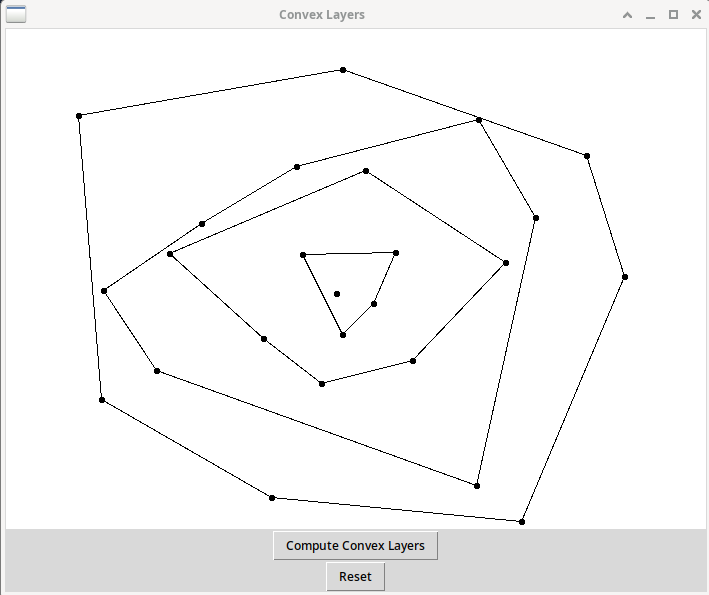
\includegraphics[width=12cm, height=9cm]{/home/arghpy/stuff/uvt/subjects/year_II/sem_I/CG/final_project/pictures/UI.png}
\newline
\newline
\subsection{Algorithm Implementation}

The Convex Layers program implements the Jarvis March algorithm, also known as the Gift wrapping algorithm, to calculate the convex hull of a set of points. The algorithm was first proposed by R. A. Jarvis in his article "On the identification of the convex hull of a finite set of points in the plane" (Jarvis, 1973)\cite{jarvis_march}.
\newline
\newline
The basic idea behind the algorithm is to start with the leftmost point and then repeatedly move counter-clockwise to the next point that is on the convex hull. This is done by considering all other points and choosing the one that is most counter-clockwise from the current point. The algorithm then proceeds with this new point and continues until it reaches the starting point again.
\newline
\newline
In our implementation, the algorithm starts by finding the leftmost point of the set of points. Then, it uses the orientation function to determine the orientation of three points, which is the current point, the next point, and another point in the set. The function returns 0 for collinear points, 1 for clockwise orientation and 2 for counter-clockwise orientation. Using this function, the algorithm finds the next point that is most counter-clockwise from the current point. The algorithm continues this process until it reaches the starting point again, and in this way, it constructs the convex hull of the points.


\subsection{Data Structures}

The program utilizes several data structures to store and manipulate the points. The primary data structure is a list of \texttt{Point objects}, which store the \textbf{x} and \textbf{y} coordinates of each point. This list is used to store all of the points that the user draws on the canvas.
\newline
\begin{lstlisting}
# Point class with x, y as point
class Point:
    def __init__(self, x, y):
        self.x = x
        self.y = y

# Create a list to hold the points drawn by the user
listPoints = []

# Function to display the point and add it to listPoints
def draw_line(event):
    x1=event.x
    y1=event.y
    x2=event.x
    y2=event.y
    listPoints.append(Point(x1, y1))
    # Draw an oval in the given co-ordinates
    canvas.create_oval(x1,y1,x2,y2,fill="black", width=5)
\end{lstlisting}
Additionally, the program uses a list of integers to store the indices of the points that make up the convex hull. This list is used to draw the lines that make up the convex hull once it has been calculated.
\newline
\newline
The program also uses a copy of the \texttt{listPoints} named \texttt{holder\_listPoints} to keep track of the points that are not in the convex hull and rules them out. This is used to draw the new convex hull once the program is run multiple times. This way the program keeps track of the points that are not in the current convex hull.
\newline
\begin{lstlisting}
# Make the copy
holder_listPoints = []
holder_listPoints = listPoints.copy()
for index in range(len(hull)):
    if index != (len(hull) - 1):
        canvas.create_line(listPoints[hull[index]].x,\
        listPoints[hull[index]].y,\
        listPoints[hull[index + 1]].x,\
        listPoints[hull[index + 1]].y)
        holder_listPoints.remove(listPoints[hull[index]])
    else:
        canvas.create_line(listPoints[hull[index]].x,\
        listPoints[hull[index]].y,\
        listPoints[hull[0]].x,\
        listPoints[hull[0]].y)
        holder_listPoints.remove(listPoints[hull[index]])
listPoints = holder_listPoints.copy()
convexHull_2(listPoints, len(listPoints))

\end{lstlisting}

\noindent The data structures are implemented in such a way that they are easy to update and manipulate as the user adds and removes points. The use of the \texttt{Point class} and the list of indices also allows for easy integration with the Jarvis March algorithm for convex hull calculation, as described in Jarvis (1973) \cite{jarvis_march}.

\section{Evaluation and Results}

\section{Applications and Future Work}

\section{Conclusion}

\bibliography{references.bib}{}
\bibliographystyle{plain}
\end{document}

